\documentclass[12pt]{article}
\usepackage[top=1in,bottom=1in,left=1in,right=1in]{geometry}
\usepackage{alltt}
\usepackage{array}	
\usepackage{graphicx}
\usepackage{tabularx}
\usepackage{verbatim}
\usepackage{setspace}
\usepackage{listings}
\usepackage{amssymb,amsmath, amsthm}
\usepackage{qtree}
\usepackage{hyperref}
\usepackage{oz}
\usepackage[cc]{titlepic}
\usepackage{fancyvrb}
\usepackage{epstopdf}
\usepackage{soul}
\graphicspath{ {./figures/} }

\newcolumntype{L}{>{\centering\arraybackslash}m{3cm}}

\title{Concordia University\\
Department of Computer Science and Software Engineering\\
\textbf{SOEN 331 - S\\Formal Methods for Software Engineering}\\
\ \\
\textbf{Assignment 3: \\Extended Finite State Machines}}
\author{\textbf{Witnick-Hans Joseph}\\
		\texttt{ID: 29348743}\\
		\textbf{Alexandra Zana}\\
		\texttt{ID: 40131077}\\
		\textbf{Alexandre Eid}\\
		\texttt{ID: 40155833}
\ \\}
\date{October 28, 2021.}

\begin{spacing}{1.5}
\begin{document}
\maketitle

\newpage
\tableofcontents
\newpage

\section{General information}

\noindent \textbf{Date posted}: Thursday 28 October, 2021.\\
\noindent \textbf{Date due}: Thursday, 11 November, 2021, by 23:59.\\
\noindent \textbf{Weight}: 15\% of the overall grade.

\section{Introduction}
You should form a team of \textbf{three} members. Each team should designate a leader who will submit the assignment electronically. In case you cannot find a team, please contact me and I will assign you to one.

\section{Ground rules}

This is an assessment exercise.  You may not seek any assistance while expecting to receive credit. \textbf{You must work strictly within your team and seek no assistance for this assignment ((e.g. from the teaching assistants, fellow classmates and other teams or external help)}. Please note that you should \textbf{not} discuss the assignment during tutorials. I am available to discuss clarifications in case you need any.

\noindent \textbf{All team members are expected to work relatively equally on each problem}. The team leader has the responsibility to ensure that the team does not violate this rule. \textbf{In your submission, you must include only the names of those team members who contributed to the assignment.} Accommodating someone who did not contribute will result in a penalty.

\noindent If there is any problem in the team (such as lack of contribution, etc.), the team leader must contact the instructor as soon as the problem appears.

\noindent 
\newpage

\section{System description}


\section{Your assignment}
\noindent Produce a \textbf{UML state diagram} (i.e. only the visual part of the extended finite state\\
machine) that captures the expected behavior of the system

\begin{figure}[ht]
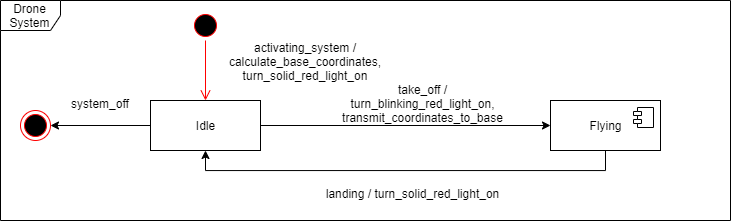
\includegraphics[width=\textwidth,keepaspectratio]{1-DroneSys.png}
\end{figure}

\begin{figure}[ht]
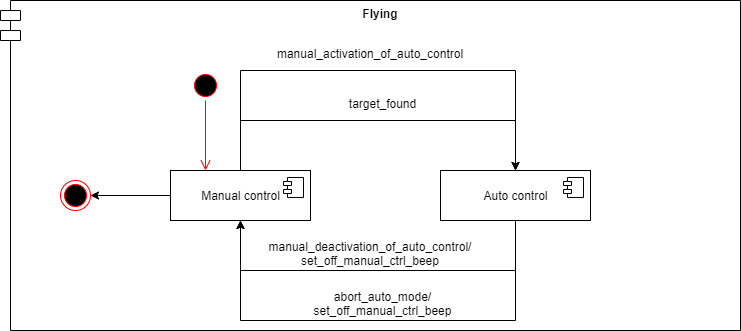
\includegraphics[width=\textwidth,height=\textheight,keepaspectratio]{2-Flying.png}
\end{figure}


\begin{figure}[ht]
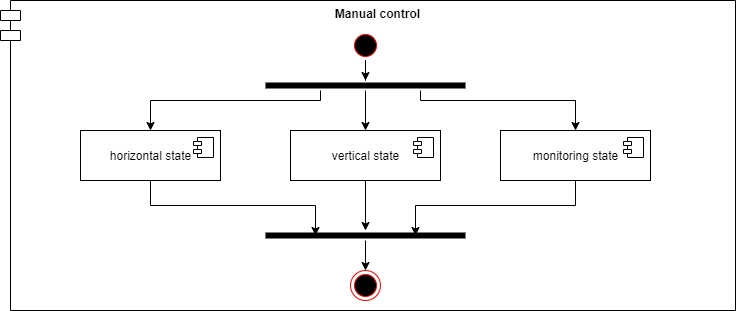
\includegraphics[width=\textwidth,keepaspectratio]{3-ManualControl.png}
\end{figure}

\begin{figure}[ht]
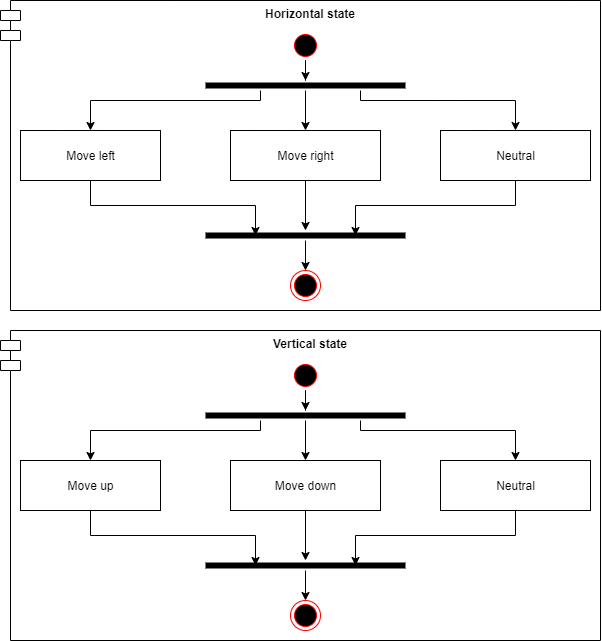
\includegraphics[width=\textwidth,keepaspectratio]{4-VertHorz.png}
\end{figure}

\begin{figure}[ht]
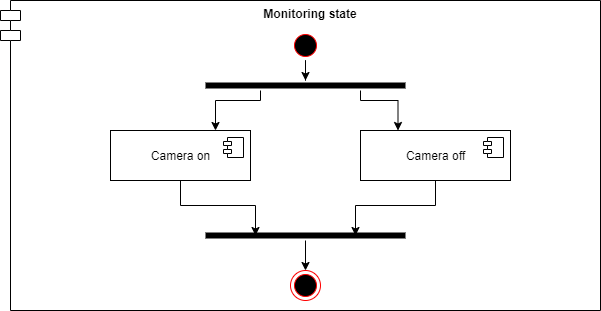
\includegraphics[width=\textwidth,keepaspectratio]{5-Monitor.png}
\end{figure}

\begin{figure}[ht]
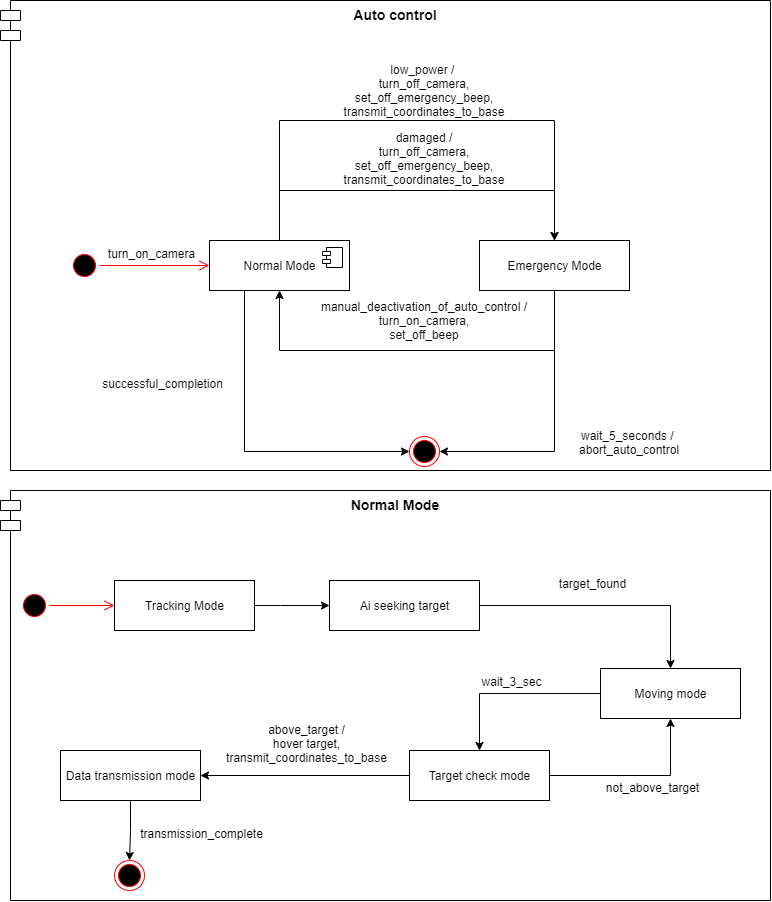
\includegraphics[width=\textwidth,height=\textheight,keepaspectratio]{6-AutoControl.png}
\end{figure}

\end{spacing}

\end{document}